% This text is proprietary.
% It's a part of presentation made by myself.
% It may not used commercial.
% The noncommercial use such as private and study is free
% Sep. 2005 
% Author: Sascha Frank 
% University Freiburg 
% www.informatik.uni-freiburg.de/~frank/



\pdfminorversion=5
\pdfobjcompresslevel=3 
\pdfcompresslevel=9

% Full presentation (with overlays, animated bullet items etc)
\documentclass[xcolor={x11names,svgnames,dvipsnames}]{beamer}

% Transparency mode (no overlays)
%\documentclass[xcolor={x11names,svgnames,dvipsnames},trans]{beamer}

% 4-up handout mode
%\documentclass[xcolor={x11names,svgnames,dvipsnames},handout]{beamer}

\usepackage{pgfpages}

\usepackage[british]{babel}
\usepackage{etex}

%% Glossy pretty look for the presentation and transparency (w/o overlays and animations) versions!
\mode<beamer|trans>{
	\useoutertheme[glossy]{wuerzburg}
	\useinnertheme[shadow,outline]{chamfered}
	\usecolortheme{shark}
}
\setbeamertemplate{navigation symbols}{}
\setbeamertemplate{frametitle continuation}[from second][(cont'd)]
\usefonttheme[stillsansseriftext,stillsansserifsmall]{serif}

%% Save up on ink for the 4-up handouts
\mode<handout>{
	\useoutertheme{wuerzburg}
	\useinnertheme[outline]{chamfered}
	\pgfpagesuselayout{4 on 1}[a4paper, landscape, border shrink=10mm]
	\pgfpageslogicalpageoptions{1}{border code=\pgfstroke}
	\pgfpageslogicalpageoptions{2}{border code=\pgfstroke}
	\pgfpageslogicalpageoptions{3}{border code=\pgfstroke}
	\pgfpageslogicalpageoptions{4}{border code=\pgfstroke}
}

\mode<presentation>{\AtBeginSection{%
		\begin{frame}
			\frametitle{Contents}
			\tableofcontents[currentsection]
		\end{frame}}}
		
		\usepackage{microtype}
		\usepackage[utf8]{inputenc}
		\usepackage[T1]{fontenc}
		\usepackage[osfss]{libertine}
		\usepackage[scaled=.77]{beramono}
		\usepackage{cmap}
		
		\usepackage{relsize,tabularx}
		\usepackage[T1,safe]{tipa}
		\usepackage{dtklogos,hologo,textcomp}
		\usepackage{multicol,booktabs}
		\usepackage{listings}
		\lstset{upquote,keepspaces=true,columns=spaceflexible,
			basicstyle=\ttfamily\scriptsize,%
			breaklines=true,breakindent=0pt,xleftmargin=0pt, xrightmargin=6pt,%
			language=[LaTeX]TeX, texcsstyle=*\bfseries\color{Maroon}, commentstyle=\sffamily\itshape\smaller\color{SeaGreen4},
			emphstyle=\bfseries\color{RoyalBlue3},escapechar={:},
			emphstyle={[2]{\bfseries\color{Sienna2}}},
			postbreak=\mbox{{\smaller\color{gray}$\hookrightarrow$}}
		}
		
		\usepackage{tikz}
		\usetikzlibrary{shapes,arrows,positioning,matrix,chains,backgrounds,fit}
		
		\usepackage{multicol}
		\usepackage[version=3]{mhchem}
		\usepackage{chemfig}
		\usepackage{linguex,qtree}
		\let\fg\lingfg
		\usepackage{texshade}
		\usepackage[detect-all]{siunitx}
		\usepackage[siunitx]{circuitikz}
		\usepackage{bytefield}
		\usepackage{auto-pst-pdf}
		\usepackage{pstricks,pst-barcode}
		\usepackage{pgfplots}
		\usepackage{pgfgantt}
		\usepackage[skaknew]{chessboard,skak}
		\usepackage{cwpuzzle}
		\usepackage{gchords,guitar}
		\usepackage{spreadtab}
		\usepackage{ccicons}


\setlength\fboxsep{0pt}
\SetTracking{encoding=*}{-39}

\author[\textsc{Jian} Wang]{\textsc{Jian} Wang\\[1ex]%
{\small\url{wangjian790@gmail.com}\\[-.5ex]\url{}}\\
{\small{Financial math Ph.D Candidate}}\\
{\small{Florida State University}}\\
[0.8ex]\copyright\copyright\copyright\copyright} %\ccbyncsa}

\title{Evolution of limit order book dynamics: One machine learning high frequency trading model}
%\titlegraphic{\ccbyncsa}
\date[\textsc{HFC} 2015]{6th High Frequency data Conference 2015 }%

% Include QR code of slides URL for presentation-mode only -- so that audience
%  can snap it and download it on the spot
\mode<beamer>{\titlegraphic{\begin{pspicture}\psbarcode[scalex=.75,scaley=.75]{http://liantze.penguinattack.org/latextypesetting.html\#mosc11-slides}{eclevel=L}{qrcode}\end{pspicture}}}

\hypersetup{%
pdfauthor={Jian Wang}, %% the "author" field from above includes garbage code...
pdfkeywords={HFC,Machine Learning,general}
}
\begin{document}
\begin{frame}
\maketitle
\end{frame}

%\title{Simple Beamer Class}   
%\author{Sascha Frank} 
%\date{\today} 

\frame{\frametitle{Table of contents}\tableofcontents} 

\section{Brief summary}
\begin{frame}
\begin{itemize}
	\item Our main goal is to use boosting machine learning method to predict the limit order book price \alert{cross over} opportunity.  	
	\item Use the high frequency data to predict relatively \alert{long time} future price changing trend.
     \item Features selection: choose what kind of data as our independent variables(\alert{choose $x_i$ s}).  
   	\item Compare the accuracy rate and calculation time  among different machine learning methods, and show that the boosting method can improve the \alert{predicting performance} to some extent.  	
\end{itemize}
\end{frame}
\section{High frequency trading}
\begin{frame}


\begin{block}{High frequency trading}
High frequency trading is a specialized case of algorithmic trading involving the \alert{frequent turnover} of many \alert{small positions} of a security.
\end{block}

\begin{columns}
\column{2.3in}
\begin{block}{Positive impact }
\begin{itemize}
\item Increased liquidity
\item Narrowing spreads
\item Improve market efficiency
\item Increase fees for Exchanges  
\end{itemize}
\end{block}

\column{2.3in}
\begin{block}{Negative impact }
\begin{itemize}
\item Impact on the institutional investors.
\item Increase volatility 
\item Disadvantages to the small Investors(\alert{asymmetric information})
\end{itemize}
\end{block}
\end{columns}

\end{frame}

\begin{frame}

\textbf{\large{HFT Strategies:}}

\begin{columns}
\column{2.4in}
\begin{block}{Market Making}
\small{place bets on both sides of the trade by placing a limit order to
sell slightly above the current market price, or to buy slightly below the current
market price, thereby profiting from the difference between the two. }
\end{block}
\begin{block}{Liquidity Rebate Trading
 }
\small{look for large orders, fill a
part of that order, and then offer these shares back to the market by placing a limit order, which makes them eligible to collect the rebate fee for providing liquidity,with or without them making a capital gain.}
\end{block}
\column{2.5in}
\begin{block}{\alert{Statistical Arbitrage}}
\small{Firms and traders looking to make profits from market arbitrage essentially exploit
 the momentary \alert{inconsistencies} in factors such as rates, prices, and other conditions
 between different exchanges or asset classes}
\end{block}
\begin{block}{Momentum Ignition }
\small{ignition strategies involve initiating and canceling a number of trades and orders with a certain security in a particular direction, which may ignite a rapid market price movement.}
\end{block}
\end{columns}
\end{frame}

\section{DataSet}
\begin{frame}
\frametitle{Dataset}
\begin{block}{Limit order book data}
The dataset contains limit order book prices of specific stock from NASDAQ. For each stock, it divided into two major components: the \alert{message book and the order} book.\\
\begin{itemize}
\item Message book: Contains Time, Prices, Volume, Event Type, Direction

\item Order book: Contains price levels, price and volume in each level for every event.  	
\end{itemize}
More details can be found in the following two charts.
\end{block} 

\end{frame}

\begin{frame}
\textbf{Message Book:}
 \begin{figure}
     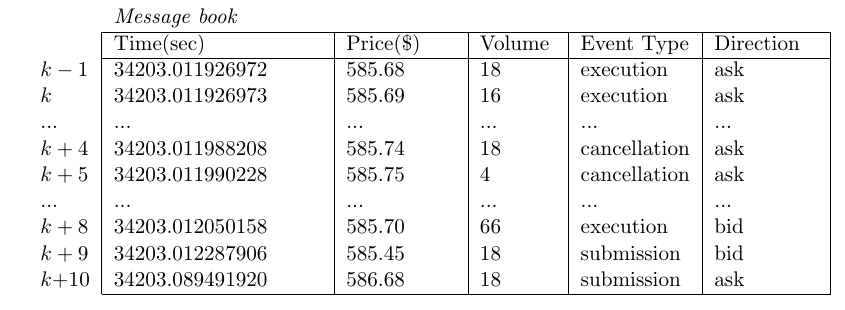
\includegraphics[width=1\textwidth, height=0.5\textheight]{message_book.png}
\end{figure}
Time is in sec and minimum time change is \alert{nanosecond}, Price is in dollars and each tick is one cent, 7 Event type, such as execution, cancellation and so on, 2 Direction ask and bid. 
\end{frame}


\begin{frame}
	\textbf{Order Book:}
	\begin{figure}
		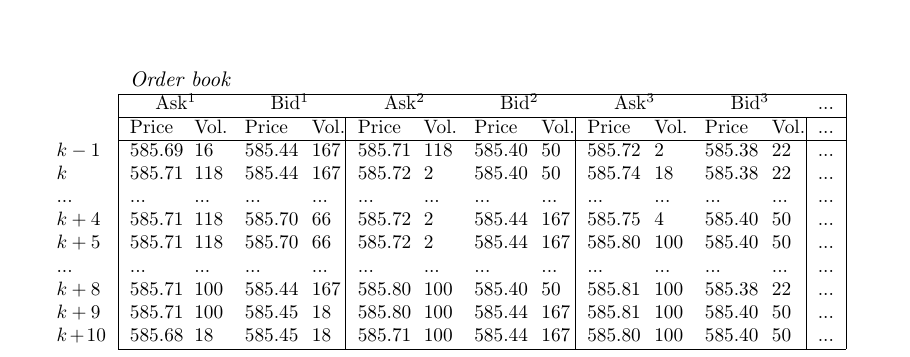
\includegraphics[width=1\textwidth, height=0.5\textheight]{order_book.png}
	\end{figure}
From level \alert{1 to level 10}, where the first level is the best bid and ask.	
\end{frame}



\section{Methodology}

\begin{frame}
\frametitle{Methodology}
%
%\setbeamercovered{transparent}
%\begin{block}{Stock Return series}
%\begin{equation}
%R_t = ln( S_{t+1})-ln(S_t)
%\end{equation}
%Where $R_t$ is the stock return at trading day t and $S_t$ is the closing price of stock at trading day t.
%\end{block}
%\setbeamercovered{transparent}
\begin{block}{Logistic regression}
\begin{center}
$ln{\frac{F(x)}{1-F(x)}}=\beta_0+\sum_i\beta_ix_i$\\
\end{center}
\end{block}

\begin{block}{Ridge regression}
\begin{center}
$\hat{\beta}^{ridge}=argmin_{\beta}\{\sum_{i=1}^p{(y_i-\hat{y_i})^2}+{\color{red}\lambda \sum_{j=1}^p\beta_j^2}\}$
\\
\end{center}
\end{block}

\begin{block}{Lasso regression}
\begin{center}
$\hat{\beta}^{lasso}=argmin_{\beta}\{\sum_{i=1}^p{(y_i-\hat{y_i})^2}+{\color{red}\lambda\sum_{j=1}^p |\beta_j|}\}$\\
\end{center}
\end{block}

\end{frame}


\begin{frame}
\frametitle{Methodology}
Comparison of L1 and L2 Penalized Model \\
\begin{columns}
\column{2.3in}
	\begin{block}{Ridge regression}
$\hat{\beta}^{ridge}=argmin_{\beta}\{\sum_{i=1}^p{(y_i-\hat{y_i})^2}+{\color{red}\lambda \sum_{j=1}^p\beta_j^2}\}$

\end{block}
\textbf{Coefficients}:
 \begin{figure}
     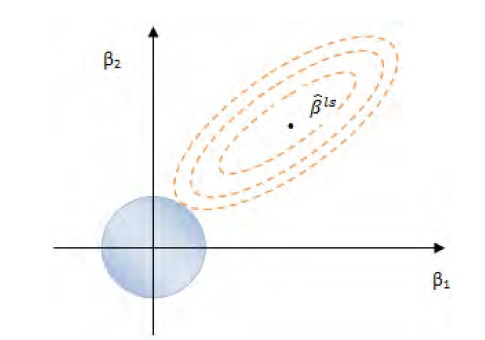
\includegraphics[width=0.9\textwidth, height=0.42\textheight]{ridge.jpg}

    \end{figure}

\column{2.3in}
\begin{block}{Lasso regression}

$\hat{\beta}^{lasso}=argmin_{\beta}\{\sum_{i=1}^p{(y_i-\hat{y_i})^2}+{\color{red}\lambda\sum_{j=1}^p |\beta_j|}\}$

\end{block}

\textbf{Coefficients}:
 \begin{figure}
     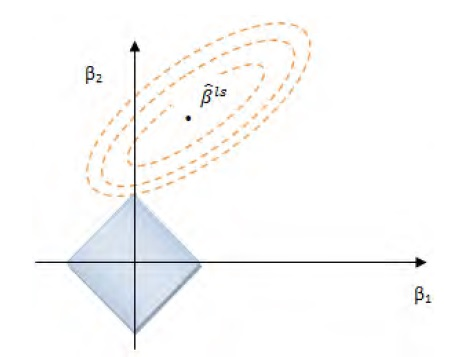
\includegraphics[width=0.9\textwidth, height=0.42\textheight]{lasso.jpg}
    \end{figure}
\end{columns}


\end{frame}

\begin{frame}
\frametitle{Methodology}
Comparison of L1 and L2 Penalized Model \\
\begin{columns}
\column{2.3in}
	\begin{block}{Ridge regression}
$\hat{\beta}^{ridge}=argmin_{\beta}\{\sum_{i=1}^p{(y_i-\hat{y_i})^2}+{\color{red}\lambda \sum_{j=1}^p\beta_j^2}\}$

\end{block}
\textbf{Path:}:
 \begin{figure}
     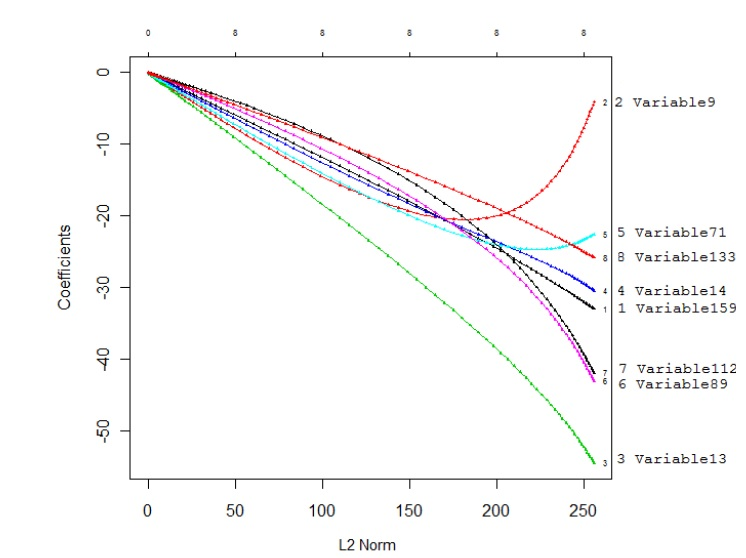
\includegraphics[width=0.8\textwidth, height=0.45\textheight]{ridge_p.jpg}

    \end{figure}

\column{2.3in}

\begin{block}{Lasso regression}

$\hat{\beta}^{lasso}=argmin_{\beta}\{\sum_{i=1}^p{(y_i-\hat{y_i})^2}+{\color{red}\lambda\sum_{j=1}^p |\beta_j|}\}$

\end{block}

\textbf{Path:}:
 \begin{figure}
     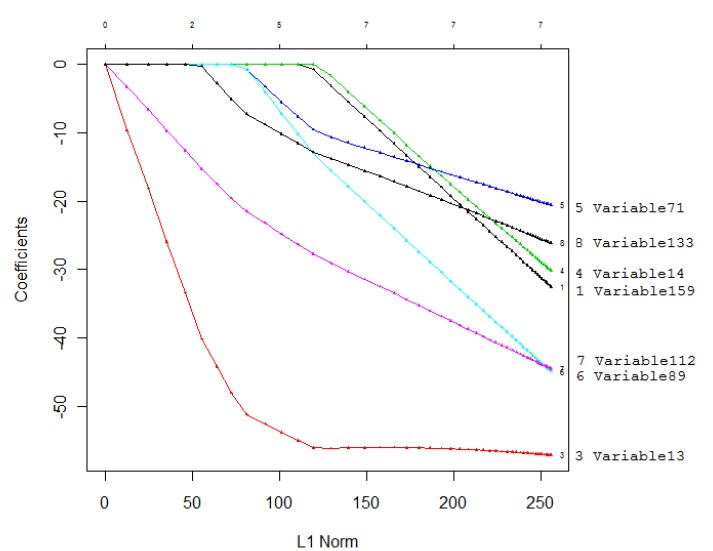
\includegraphics[width=0.8\textwidth, height=0.45\textheight]{lasso_p.jpg}

    \end{figure}
\end{columns}

\end{frame}

\begin{frame}
\frametitle{Methodology}
\begin{block}{Support vector machine}
{\small
• Introduced in COLT-92 by Boser, Guyon \& Vapnik. Became
rather popular since.\\
• Theoretically well motivated algorithm: developed from Statistical
Learning Theory (Vapnik \& Chervonenkis) since the 60s.\\
• Empirically good performance: successful applications in many
fields (bioinformatics, text, image recognition, . . . )\\
}
\end{block}

\begin{columns}<+->
\begin{column}{0.6\textwidth}
\small {
Try to maximize the margin:\\ 
$r=1/||w||,y_j=1,-1$\\
\alert{primal form}:\\
$\max\limits_{W,b}\ r= 1/||W||$\\
$s.t.(W^Tx_j+b)y_j>=1$\\
\alert{Dual form}:\\
$\max\limits_{\alpha_1,...,\alpha_M}\ \sum\alpha_l-\frac{1}{2}\sum_{j=1}^{M}\sum_{k=1}^{M}\alpha_j\alpha_k y_j y_k<X_j,X_k>$\\
s.t.$\alpha_l\geq 0$, $\sum_{l=1}^{M}\alpha_ly_l=0$
}
\end{column}
\begin{column}{.4\textwidth}
     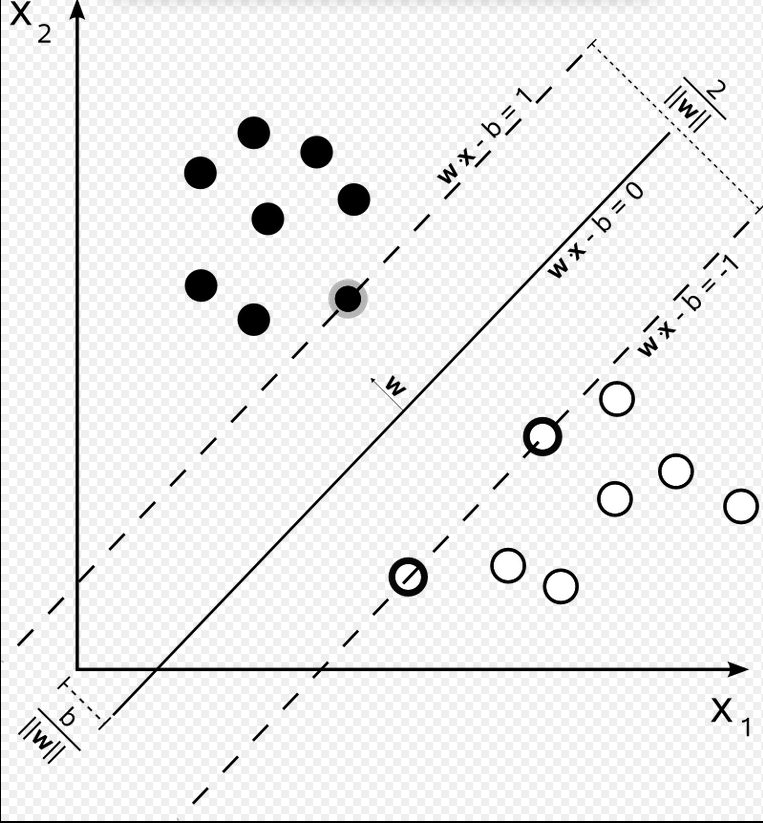
\includegraphics[width=0.8\textwidth, height=0.4\textheight]{svm.png}
\end{column}
\end{columns}
\end{frame}

\begin{frame}
\frametitle{Methodology}
\setbeamercovered{transparent}
\begin{block}{Kernel functions}
We can use the kernel function to calculate the inner product in high dimensional cases in its original feature spaces.
\end{block}
\begin{block}{Example:two dimension polinomial}
$k(x,z)=(x^Tz)^2$\\
$=(x_1^2,\sqrt{2}x_1x_2,x_2^2)^T(z_1^2,\sqrt{2}z_1z_2,z_2^2)$\\
$=\Phi(x)^T\Phi(z)$\\
\end{block}
\begin{block}{Kernel functions that we used}
\small{
\textbullet\ {Linear kernel:  $k(x,y)=x^Ty+c$}\\
\textbullet\ {Polynomial Kernel:  $k(x,y)=(\alpha x^Ty+c)^d$}\\
\textbullet\ {Radial basis function kernel(RBF):  $k(x,y)=exp(-\gamma||x-y||^2)$}
}
\end{block}
\end{frame}

\begin{frame}
	\frametitle{Methodology}
	\setbeamercovered{transparent}
	\begin{block}{Boosting methods}
	  \begin{itemize}
	  \item Introduced in 1990s
	  \item Originally designed for classification problems
	  \item Later extended to regression
	  \item Motivation - a procedure that \alert{combines the outputs of many “weak” classifiers to produce a powerful “committee”}	  
	  \end{itemize}
	\end{block}
\end{frame}

\begin{frame}
	\frametitle{Methodology}
	\setbeamercovered{transparent}
	\begin{block}{Boosting methods}
      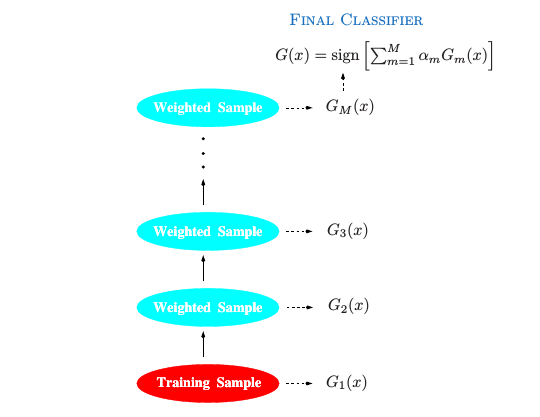
\includegraphics[width=0.8\textwidth, height=0.7\textheight]{boosting.png}
	\end{block}	
\end{frame}

\begin{frame}
	\frametitle{Methodology}
\begin{columns}

	\begin{column}{.5\textwidth}
		\textbf{Adaboosting algorithm:}\\
		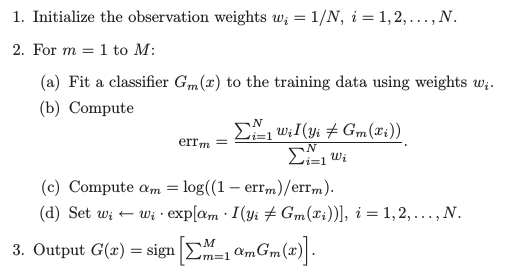
\includegraphics[width=1\textwidth, height=0.5\textheight]{adaboosting.png}\\
		\small{\textbf{source:ESL}}\\
		\alert{\textbullet\ Put more weights on the false classification data}
	\end{column}
	\begin{column}{.5\textwidth}
		\textbf{Gradient tree boosting algorithm:}\\
		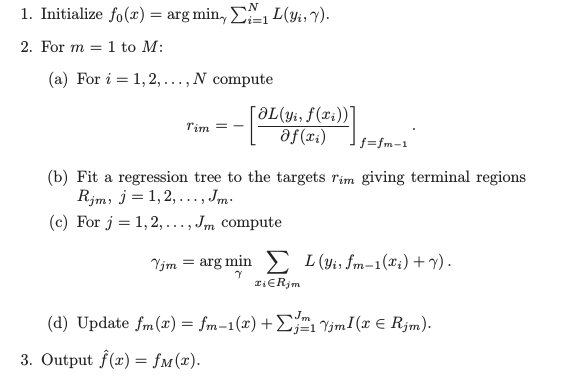
\includegraphics[width=1\textwidth, height=0.5\textheight]{gradientboost.png}\\
	    \small{\textbf{source:ESL}}\\
	    \alert{\textbullet\ Use gradient descent methods to minimize the residual in each step}
	\end{column}
\end{columns}	
\end{frame}

\begin{frame}
	\begin{block}{Boosting methods error rate evolution}
		\footnotesize{
      Boosting method can dramatically increase the performance of even a very weak classifier.We further implement the figure 10.2 in the ESL for example. Suppose features $X_1, X_2,...,X_10$ are standard independent Gaussian, and the deterministic target $Y$ is defined by:\\
      \begin{equation*}
       Y=\left\{
       \begin{array}{l}
       1\ \quad\quad if \sum_{j=1}^{10}X_j^2>\chi_{10}^2(0.5) \\
       -1\ \quad otherwise\\
       \end{array}
       \right.    
      \end{equation*} 
    where $\chi_{10}^2(0.5)$ is the median of a chi square random variable with 10 degrees of freedom.}
	\end{block}
	\begin{columns}		
		\begin{column}{.6\textwidth}
			\begin{center}
						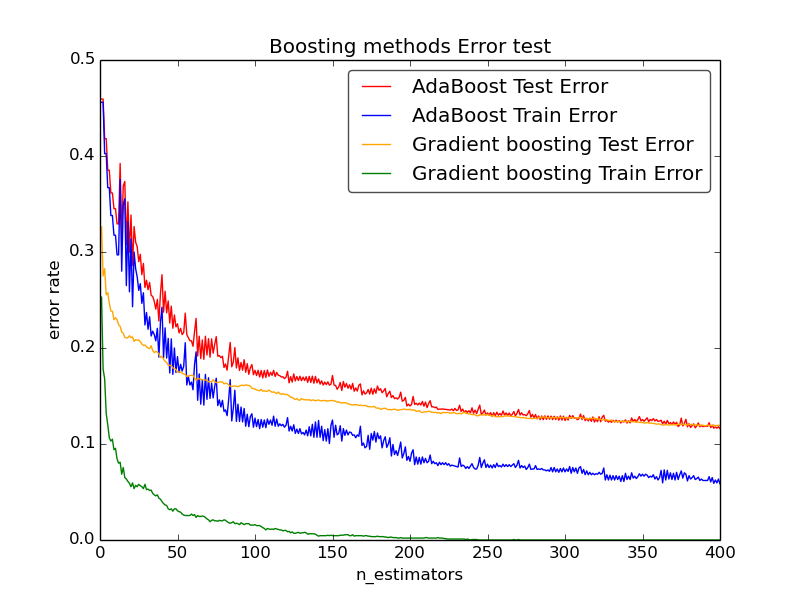
\includegraphics[width=0.8\textwidth, height=0.45\textheight]{boosting_error.png}
			\end{center}
		\end{column}
		\begin{column}{.4\textwidth}
			\begin{itemize}
				\small{
			\item Boosting methods can reduce the prediction error rate to around one third of the original.
			\item In this case, Gradient boosting method performance better}
			\end{itemize}
		\end{column}
	\end{columns}	
\end{frame}
\section{Model fit}

\newcommand<>{\hover}[1] {\uncover#2 {
	\begin{tikzpicture}[remember picture,overlay,fill opacity=1]
    \draw [fill opacity=1] (current page.south west)
	rectangle (current page.north east);
	\node at (current page.center) {#1};
	\end{tikzpicture}}
	}

\begin{frame}
\frametitle{Model built}
\begin{columns}		
		\begin{column}{.5\textwidth}
		   \textbf{order book snapshot:}\\
			\begin{center}
						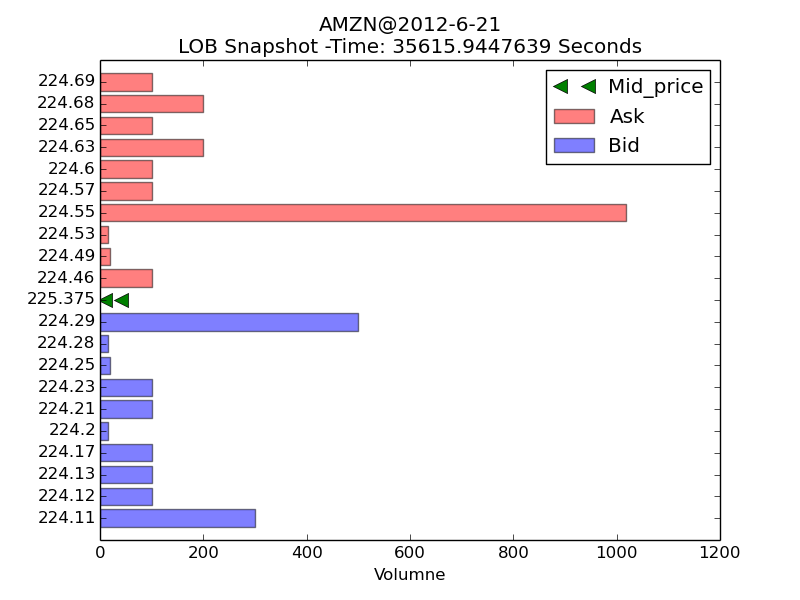
\includegraphics[width=1\textwidth, height=0.5\textheight]{orderbook_example.png}
			\end{center}
		\end{column}
		\begin{column}{.5\textwidth}
			\begin{itemize}
			\item At Time t: $P_t^A>P_t^B$, no arbitrage 
			\item At Time t+ $\Delta t$, there are three situations:\\
			\subitem \textbullet $P_{t+\Delta t}^A<P_t^B$: \alert{ask lower},denote as 1 in our model
			\\
			\subitem\textbullet  $P_{t+\Delta t}^B>P_t^A$: \alert{bid higher}, denote as -1 in our model
			\\
			\subitem\textbullet  otherwise(implies that\alert{no direction} change)
			\end{itemize}
		\end{column}
	\end{columns}
	\hover<2>{
	      \begin{minipage}{0.8\linewidth}
	        \begin{block}{Our major concern is:}
	        \alert{Cross over opportunities}, that is bid higher or ask lower after some time.
	        \end{block}
	      \end{minipage}
	      }	
\end{frame}



\begin{frame}
\frametitle{Arbitrage Numbers:}
\begin{block}{Five stocks arbitrage numbers:}
\begin{table}[h!]\small
  \caption{Arbitrage numbers based on time lag(seconds):}
\begin{center}
    \begin{tabular}{|c|c|c|c|c|c|}
    \hline
    Time&	AAPL &	AMZN&	GOOG&	INTC&	MSFT    \\
    &	(400391) &	(269748)&	(147916)&	(624040)&	(668765)  \\  
    \hline
    \small{
1s&	14926&	3423&	1269&	5752&	10198\\
5s&	52929&	13401&	5920&	29660&	32948\\
10s&	86149&	26533&	10463&	48113&	64820\\
15s&	108547&	38231&	14070&	70779&	91509\\
20s&	128771&	49684&	18218&	86649&	119450\\

}
\hline
\end{tabular}
\end{center}
\end{table}
\end{block}
From the above table, we can see that Microsoft had the largest number of events and GooGle was the least. When the time latency increased, the arbitrage numbers of all the five stocks increased 
\end{frame}




\begin{frame}
\textbf{Build features:}\\
	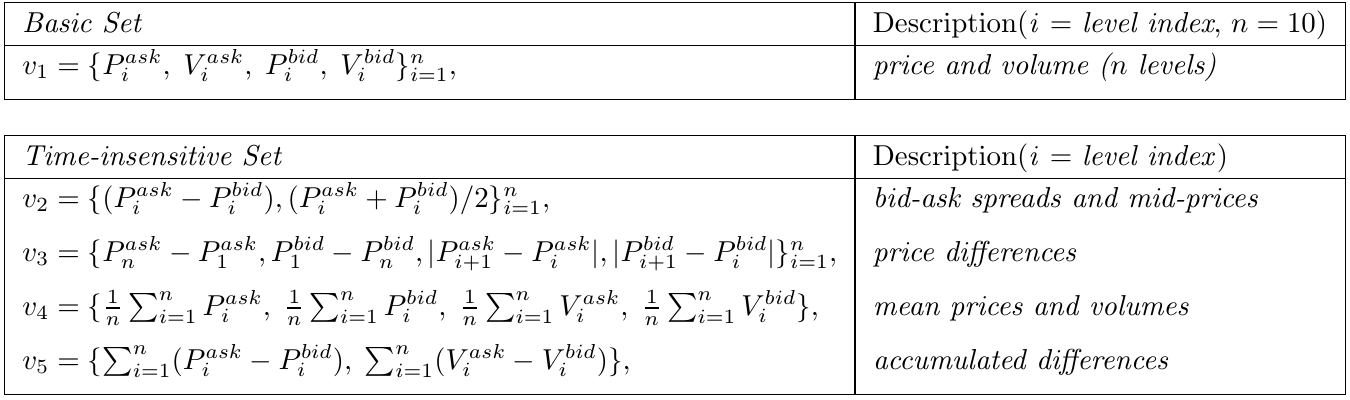
\includegraphics[width=1\textwidth, height=0.5\textheight]{features.png}
\begin{itemize}
			\item contain \alert{price,volume, bid ask spread, price difference and volume difference for each level, mean of price and volume.}  
            \item total 86 variables,  can be treated as high dimensional problems.
\end{itemize}
\end{frame}

\begin{frame}
\frametitle{Numerical results:}
\begin{block}{AAPL Predict(1 seconds):}
\begin{table}[h!]\small
  \caption{AAPL Accuracy rate and CPU time}
\begin{center}
    \begin{tabular}{|c|c|c|}
    \hline
    Methods& Accuracy rate& CPU time \\
    \hline\small{
Logistic&60.75\%&0.08\\
Ridge(alpha=1)&58.10\%&0.01\\
Lasso(alpha=0.001)&58.10\%&1.32\\
SVM&61.25\%&0.11\\
Decision tree&50.95\%&3.00\\
Ada Boosting Tree&64.85\%&39.83\\
Gradient Boosting Tree&67.05\%&16.33\\
}
\hline
\end{tabular}
\end{center}
\end{table}
\end{block}
\small{remark: \alert{training samples 8000 and test samples 2000}. The parameter for adaboosting and gradient boosting are: \alert{depth =3 and iterations =500}.Computer is 8G memory and Intel Xeon E3 processor(4 cores)}
\end{frame}


\begin{frame}
\frametitle{Numerical results:}
\begin{block}{AAPL Predict(5 seconds):}
\begin{table}[h!]\small
  \caption{AAPL Accuracy rate and CPU time}
\begin{center}
    \begin{tabular}{| c | c|c|}
    \hline
    Methods& Accuracy rate& CPU time \\
    \hline\small{
Logistic&64.70\%	&0.06\\
Ridge(alpha=1)& 63.80\%	&0.02\\
Lasso(alpha=0.001)&63.80\%	&1.28\\
SVM&65.35\%	&0.11\\
Decision tree &	62.70\%	&2.67\\
Ada Boosting Tree&	66.30\%&	32.38\\
Gradient Boosting Tree&	64.00\%	&14.84\\
}
\hline
\end{tabular}
\end{center}
\end{table}
\end{block}
\small{remark: \alert{training samples 8000 and test samples 2000}. The parameter for adaboosting and gradient boosting are: \alert{depth =3 and iterations =500}.Computer is 8G memory and Intel Xeon E3 processor(4 cores)}
\end{frame}


\section{Future work}
\begin{frame}
\frametitle{Future work}
    \begin{itemize}
        \item  Use high performance method such as parallel computing to improve the speed.
        \item  Add more meaning features.
        \item  Conduct cross validation or bagging methods.
        \item  Test the Profit and Loss(PNL) which traders mainly concern.
        \item  Try to publish in our Quantitative Finance :P
      \end{itemize}
\end{frame}

\section{Questions}

\begin{frame}
\frametitle{QA}
\begin{center}
\huge{Thanks a lot and Questions}
\end{center}
\end{frame}

\end{document}

